我们以10大小的batch进行训练,每训练10次做一次记录,总共训练1000次,得到如下的各模型的F1变化趋势,os却是收敛得最快的。

\begin{figure}[hp]
\centering
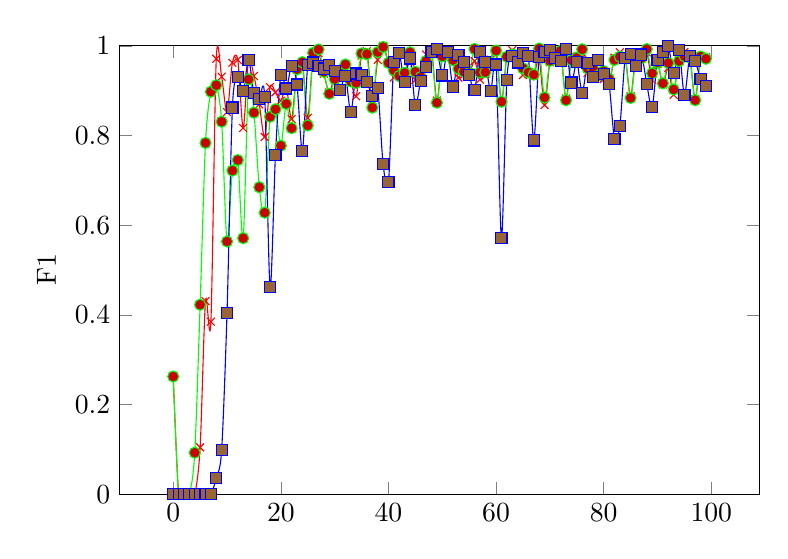
\begin{tikzpicture}
\begin{axis}[ymin=0, ymax=1, width=0.8\textwidth,
    height=0.6\textwidth, ylabel=F1]
\addplot+[smooth, color=red, mark=x]
coordinates
{
    (0, 0.2638888784891176) (1, 0.0) (2, 0.0) (3, 0.0) (4, 0.0) (5, 0.10434778489232953) (6, 0.4303796231695907) (7, 0.38461530999355525) (8, 0.9710980110532861) (9, 0.9310342398339706) (10, 0.8521735766206912) (11, 0.9621991625987134) (12, 0.9685533208419724) (13, 0.8166665636760982) (14, 0.969359208889025) (15, 0.9326423773525947) (16, 0.8693332280862199) (17, 0.7967478204378248) (18, 0.9078496886815286) (19, 0.8963854441064187) (20, 0.8774190978402231) (21, 0.9081078852538691) (22, 0.8368791631613104) (23, 0.9481479887190662) (24, 0.9627327835155256) (25, 0.8393781396173352) (26, 0.9784614017782187) (27, 0.9836955308160108) (28, 0.9376692613275919) (29, 0.8962262231669453) (30, 0.9333331846552244) (31, 0.939313871649647) (32, 0.9583330311926922) (33, 0.9204543080195401) (34, 0.8875737260604448) (35, 0.9781657449403662) (36, 0.9878047413223601) (37, 0.8787877780381227) (38, 0.9686409617552905) (39, 0.9999998792555205) (40, 0.962318713944342) (41, 0.9292033531603231) (42, 0.9323841909958122) (43, 0.9395603223737015) (44, 0.9650346586538061) (45, 0.9239763628744913) (46, 0.9319369512572139) (47, 0.9805823081632625) (48, 0.9915012889119295) (49, 0.8780486832601254) (50, 0.9767440141701176) (51, 0.9873416586702735) (52, 0.9743588325774918) (53, 0.9288701164408449) (54, 0.9352516458260466) (55, 0.9364160621005102) (56, 0.9659860962197215) (57, 0.9248552486221773) (58, 0.9365851584346321) (59, 0.96907193816599) (60, 0.991999879902067) (61, 0.8768471925891602) (62, 0.9763777782382577) (63, 0.9902437927878082) (64, 0.9614033556222988) (65, 0.934865737766901) (66, 0.937728781784539) (67, 0.9329267001377846) (68, 0.970059616523123) (69, 0.8679242804798655) (70, 0.9633025516795036) (71, 0.9753692399916503) (72, 0.9865227903286646) (73, 0.8823528429932423) (74, 0.9767440141701176) (75, 0.9759614319505278) (76, 0.9841268068282225) (77, 0.9398494636500013) (78, 0.943521452372732) (79, 0.9276314404131505) (80, 0.925925666438517) (81, 0.9139070099912975) (82, 0.9734511318822432) (83, 0.9857817784150544) (84, 0.9756096360633904) (85, 0.8872179441613224) (86, 0.9818180197292031) (87, 0.9747473629963085) (88, 0.9852939531901608) (89, 0.9236362111526577) (90, 0.9599998547202467) (91, 0.9136689155377532) (92, 0.9508194362451605) (93, 0.8907559626869064) (94, 0.9833331473197674) (95, 0.9863011653972437) (96, 0.9762531812089027) (97, 0.8804346739900207) (98, 0.9765884804780989) (99, 0.9740931496793767)
};
\addplot+[smooth, color=green, mark=*]
coordinates
{
    (0, 0.26238052831272146) (1, 0.0) (2, 0.0) (3, 0.0) (4, 0.09248552486221773) (5, 0.4225350761756142) (6, 0.7834099743467382) (7, 0.8976376883131548) (8, 0.91208768456749) (9, 0.8307690373494566) (10, 0.5635357702514674) (11, 0.7216494000957936) (12, 0.7450979563054047) (13, 0.5708884198141888) (14, 0.9251335775374346) (15, 0.850961445592332) (16, 0.6845360183961089) (17, 0.6278316229659819) (18, 0.8417720309607877) (19, 0.8584685870663258) (20, 0.77714265553016) (21, 0.8704661164813442) (22, 0.8163262784955393) (23, 0.9477610334765508) (24, 0.9634145007958821) (25, 0.8223349306244973) (26, 0.9842269883790657) (27, 0.9918697966644469) (28, 0.9418281364018525) (29, 0.8930230672410021) (30, 0.9257949044840154) (31, 0.9424082649600287) (32, 0.9583330311926922) (33, 0.9204543080195401) (34, 0.917197187001988) (35, 0.983050658345632) (36, 0.9815949553241041) (37, 0.8620688691185564) (38, 0.9859153353503979) (39, 0.9973332125897125) (40, 0.9618767047825958) (41, 0.9454543503474495) (42, 0.9328620411594659) (43, 0.9395603223737015) (44, 0.9855069221598184) (45, 0.9418602165093739) (46, 0.9304810575199216) (47, 0.9661833629726724) (48, 0.9857548582529876) (49, 0.8731706350197914) (50, 0.9763777782382577) (51, 0.9849245107650663) (52, 0.9679485771000083) (53, 0.9487177646507697) (54, 0.9420288305505697) (55, 0.9394811450940115) (56, 0.9929074817168089) (57, 0.9404759363241579) (58, 0.9411762611307051) (59, 0.9629627316484636) (60, 0.9893615826676958) (61, 0.8753055263109794) (62, 0.9756095760463162) (63, 0.9805824162175417) (64, 0.9782607086486685) (65, 0.9498067833159797) (66, 0.9407405825571986) (67, 0.9357796865922567) (68, 0.9938647538565029) (69, 0.8846151271700984) (70, 0.9665069670844573) (71, 0.9708735724388737) (72, 0.9889501522147308) (73, 0.8786406798780942) (74, 0.9679998242115039) (75, 0.9734938694058957) (76, 0.9922478874109132) (77, 0.949416174694834) (78, 0.9504949070877821) (79, 0.9337746940619022) (80, 0.9433959570433321) (81, 0.9261742144413134) (82, 0.9686096682743905) (83, 0.9758451966023991) (84, 0.9726774749740736) (85, 0.8838382825096062) (86, 0.9745452936571349) (87, 0.9721517869984231) (88, 0.9925924256902725) (89, 0.9386280050048899) (90, 0.9629628157628141) (91, 0.9163634850805895) (92, 0.9617483952824611) (93, 0.9026545045977779) (94, 0.9661015090638108) (95, 0.9767439797948461) (96, 0.9739582181832429) (97, 0.8787060919320893) (98, 0.9761090637703653) (99, 0.9711284932042903)
};
\addplot+[smooth, color=blue, mark=square*]
coordinates
{
    (0, 0.0) (1, 0.0) (2, 0.0) (3, 0.0) (4, 0.0) (5, 0.0) (6, 0.0) (7, 0.0) (8, 0.03603602129700148) (9, 0.09876537674146707) (10, 0.40449417568531276) (11, 0.8622752146872203) (12, 0.9299997888903745) (13, 0.8999998297502956) (14, 0.9682536193758229) (15, 0.8947364857809332) (16, 0.8807335781170406) (17, 0.8865975231807703) (18, 0.4615376556239558) (19, 0.7570619527087035) (20, 0.9357796216315178) (21, 0.9047615787610149) (22, 0.9541983079368849) (23, 0.9137053731870062) (24, 0.7657991272593807) (25, 0.9572647715395154) (26, 0.9626166182115568) (27, 0.9547323319144823) (28, 0.9492752061701895) (29, 0.9572647715395154) (30, 0.9444441466826532) (31, 0.9021736904422707) (32, 0.9327352361160798) (33, 0.8527128781929861) (34, 0.9382714296400946) (35, 0.9351849886234592) (36, 0.9199995823208358) (37, 0.8888883283962823) (38, 0.9051091891102655) (39, 0.73684151837626) (40, 0.6956517161950861) (41, 0.9646015761378592) (42, 0.9837835423583582) (43, 0.9195397500340222) (44, 0.9718873729975162) (45, 0.8681670758368994) (46, 0.9217389484918107) (47, 0.9519228691479259) (48, 0.9868418105095468) (49, 0.993670743314614) (50, 0.9339620641423957) (51, 0.9864251367256474) (52, 0.9090906410866801) (53, 0.9787230891208545) (54, 0.9641023396401102) (55, 0.9347823780486179) (56, 0.9008262772832656) (57, 0.9852937887333175) (58, 0.9636359659181348) (59, 0.8999995914008176) (60, 0.9583328801224433) (61, 0.5714273360590036) (62, 0.924242106359646) (63, 0.977168747199121) (64, 0.962962558162662) (65, 0.9841268068282225) (66, 0.97727247518124) (67, 0.7888444788307413) (68, 0.9756095760463162) (69, 0.9857817784150544) (70, 0.9911502433710113) (71, 0.9721113779530347) (72, 0.966666483805873) (73, 0.9930066777452208) (74, 0.9180325591332584) (75, 0.9633025516795036) (76, 0.8952377081549613) (77, 0.9612401409293221) (78, 0.9308753812825947) (79, 0.968420589829192) (80, 0.9374993349624382) (81, 0.9142854177964731) (82, 0.7924521513722262) (83, 0.8214279054862641) (84, 0.9732140884649497) (85, 0.9820356611715566) (86, 0.9545449620877928) (87, 0.9805445738651565) (88, 0.9152540964322993) (89, 0.863070376832637) (90, 0.968749770931398) (91, 0.987012696036967) (92, 0.9999998572329456) (93, 0.9400919692160857) (94, 0.9909907883292244) (95, 0.8909087232073322) (96, 0.97727247518124) (97, 0.96551702544628) (98, 0.9268290117196827) (99, 0.90983)
};
\end{axis}
\end{tikzpicture}
\caption{模型收敛比较}
\end{figure}
